% !TEX root = ./cvl.tex
\section{\hl{Selection Problem}}
\label{sec:background}

In the selection problem we select the subset of a dataset that should be displayed at a given scale of a generalized map. Below we define the basic components of the problem, and informally define the associated optimization problem.

\subsection{Geospatial records and weights}
\label{sec:records}

The dataset is assumed to consist of a set of \emph{geospatial records} drawn from a database table. The schema of a spatial record consists of a \emph{geometry} field (e.g. a point, line or polygon), a \emph{unique ID} field and any number of additional textual and numeric fields, such as ``city name'' and ``population''.

Each record is assigned a \emph{user defined weight} using CVL (see Section~\ref{sec:cvl:language}). The weight of a record models its importance, where a high weight corresponds to great importance. Any subset of records --- or all records for that matter --- may have the same weight. Therefore, the weights induce a partial order of the records.

\subsection{Legibility constraints}
\label{sec:mapconstraints}

At a given scale, a digital map will be rendered at a certain pixel resolution. Thus, for a given scale, we know the distance in pixels between geospatial locations. This gives rise to two particularly important \emph{legibility constraints}~\cite{harrie2007modelling} when generalizing a dataset for a given scale.

Firstly, the principle of constant information density~\cite{topfer1966principles} implies that the number of records that can be displayed in an area of a certain pixel size should be bounded. Assume that we divide the complete map into cells (or tiles) of, say, 256 x 256 pixels. The \emph{visibility} constraint~\cite{sarma2012fusiontables} states that each cell can contain at most $K$ visible records, where $K$ is a user defined parameter.

Secondly, records cannot be too close to each other in the map --- otherwise the user will not be able to interactively manipulate records in the map or clearly distinguish between them. The \emph{proximity} constraint states that every pair of visible records must be separated by at least $d$ pixels, where $d$ is a user defined parameter.

Importantly, these are just examples of constraints that we can model. In general, we can model any constraint that is based on a \emph{simple measure} and which is \emph{addressable by selection}. A simple measure is a function that maps a set of records to a scalar value. A constraint is violated if the measure exceeds a threshold. A constraint is ``addressable by selection'' if it can by satisfied by simply deleting an appropriate subset of the records for which the measure is exceeded.

This limitation implies that there exists constraints that we cannot model. Examples of such constraints are \emph{topological} constraints or \emph{spatial distribution} constraints. For these constraints, either we can not evaluate them using simple measure alone or we can not satisfy them by using selection alone.

The user chooses the set of constraints (compatible with our limitations) that must hold for a given map, and can even define new constraints using the CVL language, see Section~\ref{sec:cvl:language}.

\subsection{Conflict sets}
\label{sec:conflicts}

We model constraints such as visibility or proximity constraints using the notion of \emph{conflict sets}. A conflict set is a set of records that cannot all be selected, because the records would violate a constraint.

For the visibility constraint, one conflict set is generated for each cell that contains more than $K$ records. For the proximity constraint, one conflict set is generated for each pair of records that is less than $d$ pixels apart, see Figure~\ref{fig:proximity:conflict}. A record can be in several conflict sets, which is the case for point $p$ in the example shown in the figure.

\begin{figure}[htbp]
\begin{center}
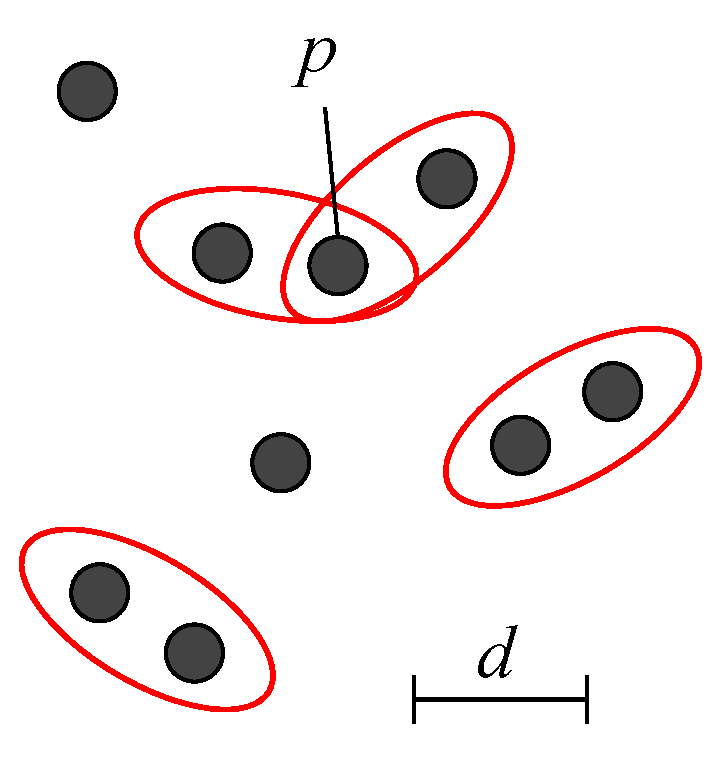
\includegraphics[scale=.3]{figs/cvl_proximity_conflicts.pdf}
\caption{Conflicts generated by the proximity constraint for distance $d$. Notice that point $p$ is a member of more than one conflict set.}
\label{fig:proximity:conflict}
\end{center}
\end{figure}


Consider a conflict set containing $k_1$ records, where at most $k_2$ of these records can be selected (where $k_1 > k_2$). Then it is equivalent to state that at least $\lambda = k_1 - k_2$ of these records must be \emph{deleted}. In the mathematical formulation of the problem in Section~\ref{sec:optimizationmodel} we will use this alternative way to formulate conflict sets.

\subsection{Filtering as an optimization problem}
\label{sec:filtering}

In the context of map generalization, the overall task of selection is to identify a subset of the dataset, such that all constraints are satisfied, and such that the aggregate weight of records that are deleted is minimized. In Section~\ref{sec:optimizationmodel} we present a mathematical formulation of this optimization problem.

\subsection{Multi-scale selection}

Besides computing a solution to the selection problem for a single scale, we are also interested in computing a series of solutions to the selection problem for a discrete set of scales or \emph{zoom levels}. This allows us to generalize a dataset for use in a zoomable map. We can select the set of zoom levels for which we compute selection, such that they correspond to the levels in the zoomable map. 

When generalizing a dataset for multiple scales, an important distinction is whether to follow the \emph{ladder} or \emph{star} approach~\cite{foerster2010challenges}. In the ladder approach, the dataset is generalized recursively, by using the output from generalization at a larger scale as the input for generalization at the next smaller scale.

We only support the ladder approach, because it automatically enforces a constraint known as the zoom-consistency constraint~\cite{sarma2012fusiontables}, which is appropriate for most datasets. The zoom-consistency constraint states that if a record is selected at a given scale, it must also be selected at all \emph{larger} scales. In other words, when a user zooms in on a map, records can only appear --- not disappear.

The star approach is appropriate for special cases like generalizing hierarchical sets of records for multiple scales. An example of this is generalizing regional labels. To illustrate this, a country label such as "Germany" should arguably be replaced by city names (e.g. ``Berlin'', ``Frankfurt'' and ``Hamburg'') at larger scales and a continent name (``Europe'') at smaller scales.

We use the term \emph{multi-scale selection} to mean the combination of a multi-scale approach, such as the ladder approach, together with using selection as the means to generalize the dataset at the individual scales.
